\chapter{Gavillas sobre $\Top$}
Dado un espacio $S$, describir sus propiedades globales puede ser una tarea complicada; en muchas ocasiones, resulta conveniente fijarse en sus propiedades locales, es decir, ver qué ocurre en una vecindad alrededor de un punto $x\in S$, por ejemplo. Así, estudiar propiedades globales de un espacio se convierte en un proceso de pasar de local a global. Intuitivamente, esto refleja algo similar a lo que ocurre con una gavilla en un espacio, ya que esta puede entenderse como una asignación $F$ que a cada abierto $U$ en $S$ se le asigna un conjunto $F(U)$, junto con una noción de ``pegado'' entre los abiertos de $S$. Dependiendo de la naturaleza del problema, en lugar de connjuntos, se pueden considerar grupos, anillos, módulos, etc., esto hace que las gavillas sean una herramienta bastante utilizada  en diversas ramas de la matemática, como topología algebraica, la geometría algebraica y, en general, en álgebra. Precisar el origen de la teoría de gavillas resulta complicado, por lo que muchos consideran un punto de partida y motivación para esta teoría el estudio de la \emph{continuación analítica}, introducida por Riemann para la comprensión de las ``funciones multivaluadas''. Aunque, cabe resaltar que, el desarrollo formal de la teoría de gavillas es gracias a Leray, Serre y Cartan. \\
En esta capítulo se presentan los conceptos fundamentales de la teoría de gavillas en conjuntos, para esto nos basamos en las ideas expuestas en \cite{maclane2012sheaves}.
\section{Gavillas sobre $\Top$}
Dado un espacio $S$, denotamos por $\O(S)$ la categoría cuyos objetos son conjuntos abiertos de $S$. Para cada par de abiertos $U$ y $V$ en $\O(S)$, $\rho:U\to V$ morfismo en $\O(S)$ si, y solo si, $U\subseteq V$.
\begin{definition}[Pregavilla]
    Una \emph{pregavilla} en $\O(S)$ es un funtor $F:\O(S)^\op\to\Con$.
\end{definition}
A un elemento $s\in F(U)$ de la imagen de un abierto $U$ de $S$ se le llama \emph{sección}. Al morfismo $F(\rho):F(V)\to F(U)$ correspondiente a la inclusión $\rho:U\hookrightarrow V$ le llamamos \emph{restricción}. Adoptamos la notación $F(\rho)(s)=s\mid_U=\rho^V_U(s)\in F(U)$ con $s$ una sección de $V$. Con esto en mente, una manera explícita en la que podemos entender una pregavilla es la siguiente: para cada par de abiertos $V\subseteq U$ de $S$ el mapeo restricción actúa como $\rho_V^U: F(U)\to F(V)$ tal que para todo $U\in\O(S)$ se  tiene que $\rho_U^U=\mathrm{id}_U$, y para cualesquiera $W\subseteq V\subseteq U\in\O(S)$ se cumple que, $\rho_W^U=\rho_W^V\circ\rho_V^U$.
\begin{lema}
    Sea $F:\O(S)^\op\to\Con$ un funtor, $U$ un abierto de $S$ y $\{U_i\}_{i\in I}$ una cubierta abierta de $U$. Entonces el diagrama 
    \begin{equation}\label{ec:2.1}
        F(U)\xrightarrow{\varepsilon}\prod_{i\in I} F(U_i)\overset{p}{\underset{q}{\rightrightarrows}}\prod_{i,j\in I}F(U_i\cap U_j),
    \end{equation}
    donde para todo $t\in F(U)$, $e(t)=\langle t\mid_{U_i}\rangle_{i\in I}$ y para toda familia $\langle t_i\in F(U_i)\rangle_{i\in I}$, $p(\langle t_i\rangle_{i\in I})=\langle t_i\mid_{(U_i\cap U_j)}\rangle_{i,j\in I}$, siempre existe y se cumple que $pe=qe$.
\end{lema}
\begin{proof}

\end{proof}
\begin{definition}[Pregavilla separada] Una pregavilla $F:\O(S)^{\op}\to\Con$ se dice \emph{separa} si la función $e$ de (\ref{ec:2.1}) es inyectiva. 
\end{definition}
\begin{definition}[Gavilla]
    Una \emph{gavilla} de conjuntos sobre un espacio topológico $S$ es un funtor $F:\O(S)^\op\to\Con$ tal que para todo conjunto abierto $U$ de $S$ existe una cubierta abierta $\{U_i\}_{i\in I}$ de tal modo que (\ref{ec:2.1}) es un igualador.  
\end{definition}
Es decir, una gavilla es pregavilla separada. En la literatura (veáse \cite{tennison1975sheaf}, por ejemplo) es común definir una gavilla como una pregavilla que satisface lo siguiente.
    \begin{enumerate}
        \item[i).] Sea $U\in\O(S)$. Si $\{U_i\}_{i\in I}$ es una cubierta abierta para $U$ y para cualesquiera dos secciones $s$ y $s'$ tales que $\rho^U_{U_i}(s)=\rho^U_{U_i}(s')$, se tiene que $s=s'$.
        \item[ii).] Sea $U\in\O(S)$ y $\{U_i\}_{i\in I}$ una cubierta de $U$. Si $\{s_i\}_{i\in I}$ es una familia de secciones de $F$, donde $s_i\in F(U_i)$, tal que  $\rho^{U_i}_{U_i\cap U_J}(s_i)=\rho^{U_j}_{U_i\cap U_j}$, para toda $i,j\in I$. entonces existe una sección $s\in F(U)$ tal que $\rho^U_{U_i}(s)=s_i$.
    \end{enumerate}
Obsérvese que la sección $s\in F(U)$ definida en ii), es única por la condición i); a esta condición ii) se le conoce comúnmente como condición de pegado. Resulta que en $\Con$, dar una pregavilla separada es equivalente a dar una pregavilla que satisface i) y ii).
\begin{definition}
    Sea $S$ un espacio topológico. La \emph{categoría de gavillas} sobre $S$ consta de lo siguiente.
    \begin{enumerate}
        \item[$\bullet$] \emph{Objetos}. Gavillas de conjuntos sobre $S$.
        \item[$\bullet$] \emph{Morfismos}. Transformaciones naturales.
    \end{enumerate}
\end{definition}
Algunos ejemplos relvantes de gavillas son los siguientes.
\begin{ejp}
\text{}
    \begin{enumerate}
        \item Sea $U\in\O(S)$. El conjunto 
        \begin{eqnarray*}
            C(U):=\{f:U\to\R\mid f\text{ es continua}\}
        \end{eqnarray*}
        es una gavilla. Para esto, primero veamos que $C(-)$ es funtorial, lo cual demostraría que en efecto es una pregavilla.
        Sea $U\overset{\rho}{\hookrightarrow} V$ con $U,V\in\O(S)$. Entonces, $C(\rho):C(V)\to C(U)$. Tomando la restricción usual, se tiene el siguiente diagrama
        \begin{figure}[H]
            \centering
            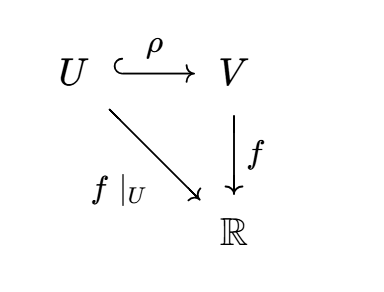
\includegraphics[width=0.25\linewidth]{img/diagram2.1.png}
        \end{figure}
        conmutativo. Esto prueba la funtorialidad, y así $C(-)$ es una pregavilla.\\
        Ahora, veamos que, para cada $U\in \O(S)$Y $\{U_i\}_{i\in I}$ una cubierta abierta para $U$, el siguiente diagrama 
        \begin{eqnarray}\label{ejp2.1}
            C(U)\xrightarrow{e}\prod_{i\in I} C(U_i)\overset{p}{\underset{q}{\rightrightarrows}} \prod_{i,j\in I}C(U_i\cap U_j)
        \end{eqnarray}
        es un igualador en $\Con$. Sea $\{f_i\}_{i\in I}\in\prod_{i\in I}C(U_i)$ tal que $p(\{f_i\})=q(\{f_i\})$. Entonces, $f_i\mid_{U_i\cap U_j}=f_j\mid_{U_i\cap U_j}$ para toda $i,j\in I$. Para cada $U\in\O(S)$, definimos la función $f:U\to\R$ de la siguiente manera
        \begin{equation*}
            f(x)=\begin{cases}
                f_i(x) & \text{si } x\in Ui,\\
                0 &\text{en otro caso.}
            \end{cases}
        \end{equation*}
        Sea $y\in (a,b)\subset\R$ tal que $f(x)=y$, para algún $x\in U$. Ya que $\{U_i\}_{i\in I}$ es una cubierta abierta para $U$, se tiene que $U=\bigcup_{i\in I}U_i$, y en particular $x\in U_i$, para algún $i\in I$. Así, $f_i(x)=f(x)=y$. Luego, como $\{f_i\}\in C(U_i)$ se sigue que $f_i$ es continua para toda $i\in I$; esto implica que existe un abierto $V\subset U_i\subset U$ tal que $x\in V$ y $f_i(V)=f(V)\subset(a,b)$. Por lo tanto, $f\in C(U)$ y $e(f)=\{f_i\}_{i\in I}$. Ahora, supongamos que existe $g\in CU$ tal que $e(g)=\{f_i\}$. Si $x\in U$ entonces, $x\in U_i$ para alguna $i\in I$. De esto se sigue que, $f(x_i)=f(x)=g(x)$. Al tener que $f$ y $g$ tienen el mismo dominio, mismo codominio y misma regla de correspondencia, así $f=g$; lo cual prueba la unicidad de $f$. Por el Lema \ref{lema:igualador}, se sigue que (\ref{ejp2.1}) es un igualador en $\Con$ y $CU$ es una gavilla. 
        \item Sea $U\in \O(S)$. El conjunto
        \begin{eqnarray*}
            C^\infty(U):=\{f:U\to\R\mid f \text{ es suave}\}
        \end{eqnarray*}
        es una gavilla. La demostración de esto es análoga a la del ejemplo anterior.
        \item Sea $U\in\O(S)$. El conjunto de funciones holomorfas
        \begin{eqnarray*}
            \Omega(U):=\{f:U\to\C\mid f\text{ es holomorfa}\}
        \end{eqnarray*}
        es una gavilla. Primero, veamos que $\Omega(-)$ es una pregavilla. Sea $U\overset{\rho}{\hookrightarrow} V$ con $U,V\in\Omega(S)$. Entonces, 
        \begin{eqnarray*}
            \Omega(\rho):\Omega(V)&\to&\Omega(U).
        \end{eqnarray*}
        Por definición, $\Omega(V)=\{f: V\to\C\mid f\text{ es holomorfa}\}$. Tomando la restricción usual, se tiene que el siguiente diagrama conmuta.
        \begin{figure}[H]
            \centering
            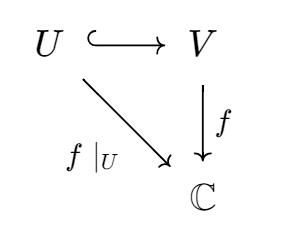
\includegraphics[width=0.2\linewidth]{img/gav3.png}
        \end{figure}
        Así, $\Omega(-)$ es funtorial y, por lo tanto, una pregavilla.\\
        Para probar que $\Omega(-)$ es una gavilla, vamos a verificar las condiciones i) y ii) dadas anteriormente.
        \begin{enumerate}
        \item[i).] Sea $U\in\O(S)$ y $\{U_i\}_{i\in I}$ una cubierta abierta para $U$. Supongamos que $s$ y $s'$ son secciones tales que $\rho^U_{U_i}(s)=\rho^U_{U_i}(s')$. Del siguiente diagrama
            \begin{figure}[H]
            \centering
            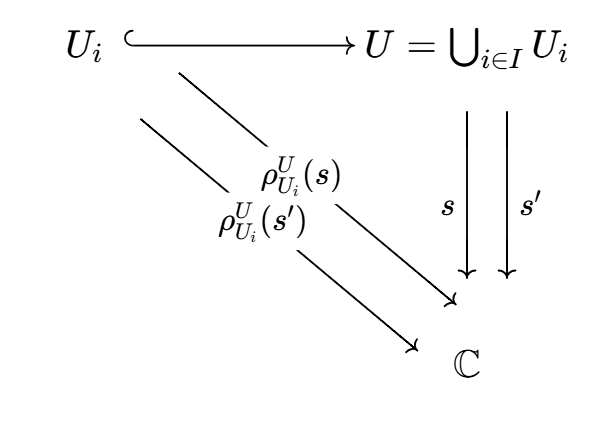
\includegraphics[width=0.4\linewidth]{img/diagram2.2.png}
        \end{figure}
        se tiene que $s=s'$.
        \item[ii).] Supongamos que $f_j:U_j\to\mathbb{C}$ son holomorfas y $f_i\mid_{U_i\cap U_j}=f_j\mid_{U_i\cap U_j}$. En $U=\bigcup_{i\in I}U_i$, definimos $f(w)=f_j(w)$, para toda $w\in U_i$. Para ver que la condición de pegado se satisface, basta verificar que $f$ satisface las condiciones de Cauchy-Riemann. Sea $z=x+iy\in\C$. Entonces, $f(z)=f(x,y)=f(x+iy)=u(x,y)+iv(x,y)$. Luego, 
   
        \begin{eqnarray*}
            \dfrac{\partial f}{\partial z}=\dfrac{\partial u}{\partial x}+i\dfrac{\partial v}{\partial y}&=& \dfrac{\partial u'}{\partial x}+i\dfrac{\partial v'}{\partial y}\quad\text{ con }u'(x,y)+iv'(x,y)=f_j(z)\\
            &=& \dfrac{\partial u'}{\partial x}=-\dfrac{\partial v'}{\partial y} \quad f_j\text{ es holomorfa}\\
            &=& \dfrac{\partial u'}{\partial x}_{u_j}=-\dfrac{\partial v'}{\partial y}_{u_j}
        \end{eqnarray*}
        Por lo tanto, $f_j=f\mid_{U_j}$. Así, $f$ es holomorfa, y $\Omega(-)$ es gavilla.
        \end{enumerate}
\end{enumerate}
\end{ejp}
\section{El funtor $\Gamma$} 
Dado $S$ un espacio topológico, la categoría de rebanadas $\Top/S$ consta de lo siguiente.
\begin{enumerate}
    \item[$\bullet$] \emph{Objetos}. Todas las funciones continuas $f\in\Mor(\Top)$ cuyo codominio son igual a $S$.
    \item[$\bullet$] \emph{Morfismos}. Para cada función continua $f:E\to E'\in\Mor(\Top)$, existen $p:E\to S$ y $p':E'\to S$ tales que $p=p'\circ f$.
    \begin{figure}[H]
        \centering
        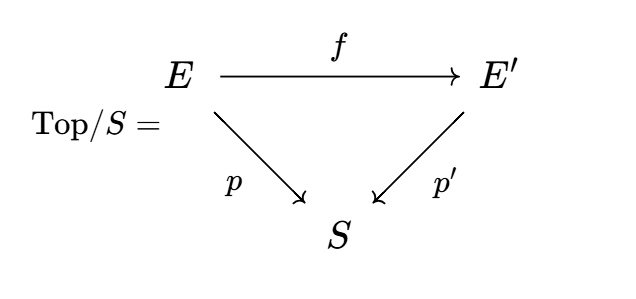
\includegraphics[width=0.42\linewidth]{img/diagram2.2.1.png}
    \end{figure}
\end{enumerate}
A una función continua de la forma $p:E\to S$ le llamamos \emph{haz} sobre $S$, y al espacio $E$ se le conoce como \emph{espacio total}. En topología algebraica es común estudiar un tipo particular de haces, los cuales se llaman haces fibrados, y no deben de confundirse con los haces que estamos estudiando ya que $f$ solo es una función continua y no un homeomorfismo; además, de que no pedimos la condición de localidad trivial como ocurre en el caso de los haces fibrados. \\
Para cada punto $x\in S$, la \emph{fibra asociada} a $x$ es la preimagen  $p^{-1}(x)$. Esto nos permite interpretar al espacio $E$ como un espacio formado por copias de cada fibra parametrizada por los puntos de $S$. Como $p:E\to S$ es una función continua, la preimagen de abiertos manda abiertos en abiertos; por lo cual, para cada $U\in S$ conjunto abierto, se tiene que $p_U:p^{-1}(U)\to U$ es un haz sobre $U$. Más aún, el siguiente diagrama
    \begin{figure}[H]
        \centering
        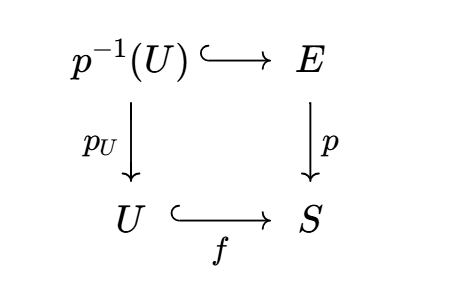
\includegraphics[width=0.32\linewidth]{img/diagram2.2.2.png}
    \end{figure}
\noindent
es un pullback en $\Top$. 
\begin{definition}[Sección] Una \emph{sección} (global) de un haz $p:E\to S$ es una función continua $s:S\to E$ tal que $p\circ s=\id_S$. Una \emph{sección local} de $p$ alrededor de $x\in S$ es una sección de $p_U$. 
\end{definition}
\begin{prop}
    Sea $p:E\to S$ un haz y $f:U\to S$ una función continua. Hay una correspondencia biyectiva entre el conjunto de secciones de $p_U$ y el conjunto de levantamientos de $f$ a $E$, es decir, funciones continuas $h:U\to E$ tal que $ph=f$.
\end{prop}
\begin{proof}
    Por la propiedad universal del pullback, dar una sección de $p_U$ es equivalente a dar un levantamiento $h:U\to E$ de $f$ que hace completar el siguiente diagrama.
        \begin{figure}[H]
        \centering
        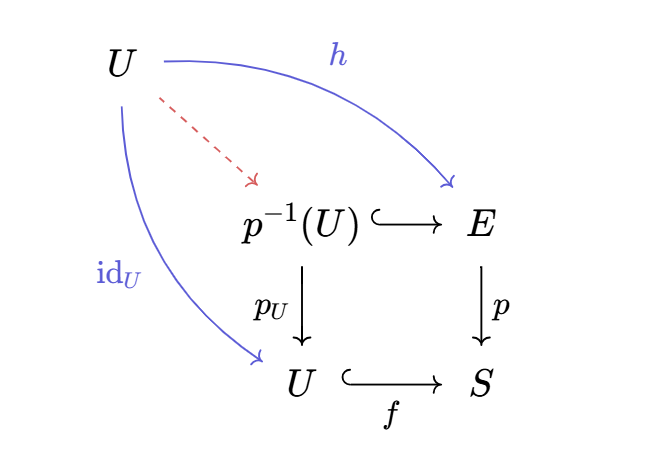
\includegraphics[width=0.43\linewidth]{img/diagram.2.2.3.png}
    \end{figure}
\end{proof}
\noindent
Denotemos por $\Gamma_pU:=\{s\mid s\text{ es una sección local}\}$. Dado un abierto $U$ de $S$ y $V\subset U$, se define
\begin{eqnarray*}
    \Gamma_pU&\to&\Gamma_p V\\
    s&\mapsto& \rho^U_V(s):=s\mid_V.
\end{eqnarray*}
\begin{lema}
    $\Gamma_p:\O(S)^{op}\to\Con$ es un funtor.
\end{lema}

\section{El funtor $\Lambda$}
Sea $P:\O(S)^{\op}\to\Con$ una pregavilla sobre un espacio un espacio $S$. Sea $x\in S$ un punto, y consideremos la familia $\O(x):=\{U\in \O(S)\mid x\in U\}$ la familia de vecindades abiertas de $x$ en $S$. Dados $U_\alpha, U_\beta\in \O(x)$ la intersección $U_\gamma:=U_\alpha\cap U_\beta\in\O(x)$ cumple que $U_\gamma\subseteq U_\alpha$ y $U_\gamma\subseteq U_\beta$. Esto es, considerando el orden pacial $\leq$ dado por la contención de abiertos, se tiene que $(\O(x),\leq)$ es un conjunto dirigido. Además, para cada morfismo  $\iota^\beta_\alpha:U_\alpha\hookrightarrow U_\beta$ en $\O(x)$, se tienen morfismos $\phi^\beta_\alpha:= P(\iota^\beta_\alpha): P(U_\beta)\to P(U_\alpha)$ los cuales forman una familia directa en $\Con$, denotada por $(P(\O(x)),\leq)$. \\
Si el colímite de $(P(\O(x)), \leq )$ en $\Con$ existe, este es denotado por $P_x:=\varinjlim P(U_\alpha)$. Para cada familia $\{M_\alpha\}$ indexada por $\O(x)$, este colímite se puede ver de manera explícita como sigue 
\begin{equation*}
     \varinjlim M_\alpha:=\left(\bigsqcup M_\alpha\right)/\sim
\end{equation*}
donde $s\sim t$ ($s\in PU$ y $t\in PV$) si, y solo si, existe un abierto $W$ tal que $W\subseteq U\cap V$ y  $s\mid_W=t\mid_W\in PW$ para $x\in W$. Además, se tienen morfismos canónicos 
\begin{eqnarray*}
    \phi:P(U_\alpha)\to\bigsqcup P(U_\alpha)\to\varinjlim P(U_\alpha).
\end{eqnarray*}
\begin{definition}[Germen]
    Dada una sección $s\in P(U)$, se define su \emph{germen} en el punto $x\in S$, denotado por $[s]_x$, como la imagen  $\phi(s)\in P_x$. 
\end{definition}
Notemos que, para un punto $x\in S$, los elementos de $P_x$ son precisamente las secciones en el punto $x$. A $P_x=\{[s]_x\mid s\in PU, x\in U\in\O(x)\}$ se le conoce como el \emph{tallo} de $P$ en $x$. 
\begin{lema}
    La relación ``$\sim$'' es de equivalencia. 
\end{lema}
\begin{proof}
\text{}
\begin{enumerate}
  \item[$\bullet$]  \emph{Reflexividad.} Sea $U\in\O(S)$ y $s\in PU$. Para $x\in U$, tenemos que $U\subseteq U$ y $s=s\mid_U$. Por lo tanto, $s\sim s$.
   \item[$\bullet$] \emph{Simetría.} Para $U,V\in\O(S)$, sean $s\in PU$ y $t\in PV$ tales que $s\sim t$. Entonces, se cumple la definición y dado que existe $W\subseteq U\cap V$, se sigue que también se cumple $t\sim s$.
    \item[$\bullet$]\emph{Transitividad.} Consideremos $U,V,W\in\O(S)$ y, $s\in PU$, $t\in PV$ y $r\in PW$ tales que $s\sim t$ y $t\sim r$. Entonces, existen $Y\subseteq U\cap V$ y $Y'\subseteq V\cap W$ vecindades de $x$ donde $s\mid_Y=t\mid_{Y}$ y $t\mid_{Y'}=r\mid_{Y'}$. Nótese que $Y\cap Y'$ es una vecindad de $x\in U\cap W$. Como $s\mid_Y=t\mid_Y$ implica que $s\mid_{Y\cap Y'}=t\mid_{Y\cap Y'}$. Además, $t\mid_{Y\cap Y'}=r\mid_{Y\cap Y'}$. Por lo tanto, $s\mid_{Y\cap Y'}=r\mid_{Y \cap Y'}$ y $s\sim r$.
    \end{enumerate}
    Ya que $\sim$ es reflexiva, simétrica y transitiva se tiene que es de equivalencia.
\end{proof}

\begin{lema}
    Sea $P^x:\O(x)\to\Con$. Las funciones $\{\germ_x: P(U)\to\O(x)\}$ tales que para cada sección $s\in P(U)$, $\germ_xs=[s]_x$, forman un cocono colímite sobre $\O(x)$. Más aún, este es filtrante.
\end{lema}
\begin{proof}
    Sean $U,V\in\O(x)$. Entonces, se tiene el siguiente diagrama
    \begin{figure}[H]
        \centering
        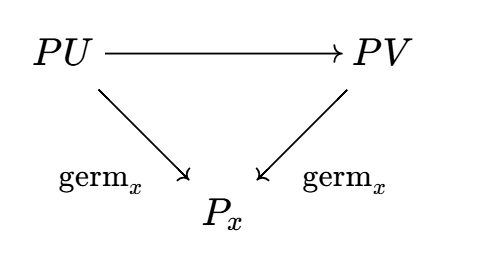
\includegraphics[width=0.3\linewidth]{img/diagram_2.3.1.png}
    \end{figure}
    Si $s\in PU$ es tal que $s\mid_V=PV$, entonces $[s]_x=[s\mid_V]_x$. Por lo tanto, el diagrama anterior conmuta y $(\germ_x:PU\to P_x)_{U\in \O(x)}$ es un cócono. Ahora, consideremos $(\tau_u: PU\to L)_{U\in\O(x)}$ otro cocono sobre $P^{(x)}$. Veamos que existe una única función $t:P_x\to L$ tal que $t\circ\germ_x=\tau$. Esto es, 
    \begin{figure}[H]
        \centering
        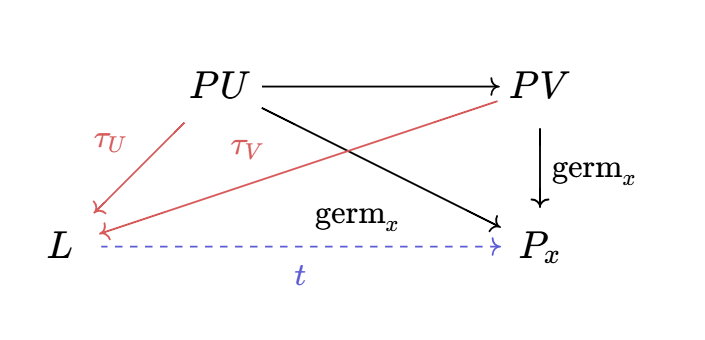
\includegraphics[width=0.45\linewidth]{img/diagram2.3.2.png}
    \end{figure}
    Definamos $t:P_x\to L$ como $t([s]_x)=\tau_U(s)$. Ahora, tomemos $r$ otro representante, i.e., $[s]_x=[r]_x$ implica que existe $W\in U\cap V$ tal que $s\mid_W=r\mid_W$ y $\tau_W(s\mid_W)=\tau_W(r\mid_W)$. Como $\tau$ es un cócono, entonces 
    \begin{eqnarray*}
    \tau_U(s)=\tau_W(s\mid_W)=\tau_W(r\mid_W)=\tau_V(r).
    \end{eqnarray*}
    Por lo tanto, $t$ está bien definida. Ahora, sea $s\in PU$. Entonces, $t\circ\germ_x(s)=t([s]_x)=\tau_U(s)$. Por otro lado, consideremos $l:P_x\to L$ tal que $l\circ\germ_x(s)=\tau$. Si $[s]_x\in P_x$, se tiene que
    \begin{eqnarray*}
        t([s]_x)&=& t\circ\germ_x(s)=\tau(s)\\
        &=& l\circ\germ_x(s)=l([s]_x).
    \end{eqnarray*}
    Por lo tanto, $t$ es única y $\{\germ_x:PU\to P_x\}$ es un cócono límite.
\end{proof}
\begin{lema}
    Cualquier morfismo $h:P\to Q$ de pregavillas (cualquier transformación natural), en cada punto $s\in S$, induce una única función $h_x:P_x\to Q_w$ tal que el diagrama 
    \begin{figure}[H]
        \centering
        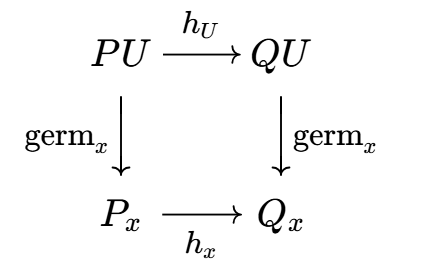
\includegraphics[width=0.3\linewidth]{img/diagram2.3.3.png}
    \end{figure}
    conmuta para cualquier $U\in\O(x)$.
\end{lema}
\begin{proof}
    Sea $h:P\to Q$ una transformación natural. Sean $U,V\in\O(x)$ tal que $V\leq U$. Si $s\in PU$, al ser $h$ natural se tiene que $\germ_x\circ h_V(s\mid_V)=\germ_x(h_V(s)\mid_V)$. Por el lema anterior, $\{\germ_x:PU\to PV\}$ es un cócono límite; así, existe una única función $h_x:P_x\to Q_x$ que hace conmutar el diagrama deseado. Además, $h_x([s]_x)=[h_U(s)]_x$. 
\end{proof}
\noindent
Del resultado anterior, tenemos el diagrama conmutativo
    \begin{figure}[H]
        \centering
        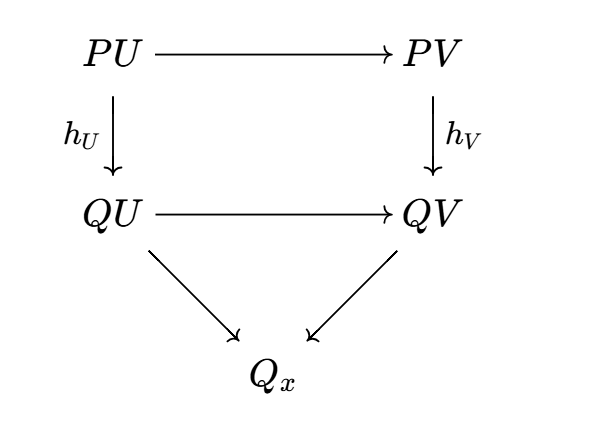
\includegraphics[width=0.37\linewidth]{img/diagram2.3.4.png}
    \end{figure}
\noindent
Un resultado inmediato es el siguiente.
\begin{lema}
    La transformación natural dada por $h\to h_x$ es un funtor de $\Con^{\O(x)}\to \Con$. Dicho funtor es ``tomar germen en $x$''.
\end{lema}
Sea 
\begin{eqnarray*}
\Lambda_p=\bigsqcup_{x\in S}P_x=\bigsqcup_{x\in S}\{[s]_x\mid s\in PU\}
\end{eqnarray*} 
la unión disjunta de germenes sobre $x\in S$. Para toda sección $s\in PU$, definamos las siguientes funciones
\begin{eqnarray*}
    p:\Lambda_p&\to& S\\
    \left[s\right]_x&\mapsto& x,\\
    \hat{s}:U&\to&\Lambda_p\\
    x&\mapsto& \left[s\right]_x.
\end{eqnarray*}
\begin{lema}
    El conjunto $B_p:=\{\hat{s}(U)\mid s\in PU, U\in\O(S)\}$ es una base para una topología en $\Lambda_p$.
\end{lema}

\section{$\H L/S\cong \Gav(S)$}

\section{Morfismos ultrafinitos}

\section{Cambio de base}